%\setchapterimage{fig_00.jpg}
\chapter*{TD \arabic{cptApplication} \\ 
Machine de forage -- \ifprof Corrigé \else Sujet \fi}
\addcontentsline{toc}{section}{TD \arabic{cptApplication} : Machine de forage -- \ifprof Corrigé \else Sujet \fi}

\iflivret \stepcounter{cptApplication} \else
\ifprof  \stepcounter{cptApplication} \else \fi
\fi

\setcounter{question}{0}
\marginnote{D'après Concours CCINP 2023 -- MP.}
\marginnote[1cm]{
\UPSTIcompetence[2]{B2-14}
\UPSTIcompetence[2]{C1-05}
\UPSTIcompetence[2]{C2-07}
}

\begin{marginfigure}
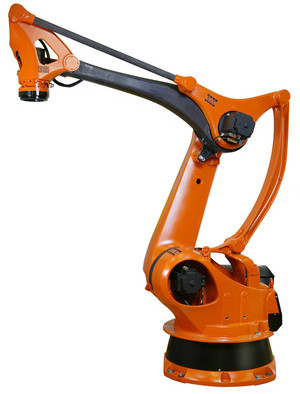
\includegraphics[width=\linewidth]{fig_01}
\end{marginfigure}


Dans le domaine du génie civil, les foreuses permettent de réaliser des perçages profonds afin de couler des pieux en béton armé. On s'intéresse aux conditions de basculement statique de la foreuse. 

\begin{marginfigure}
\centering
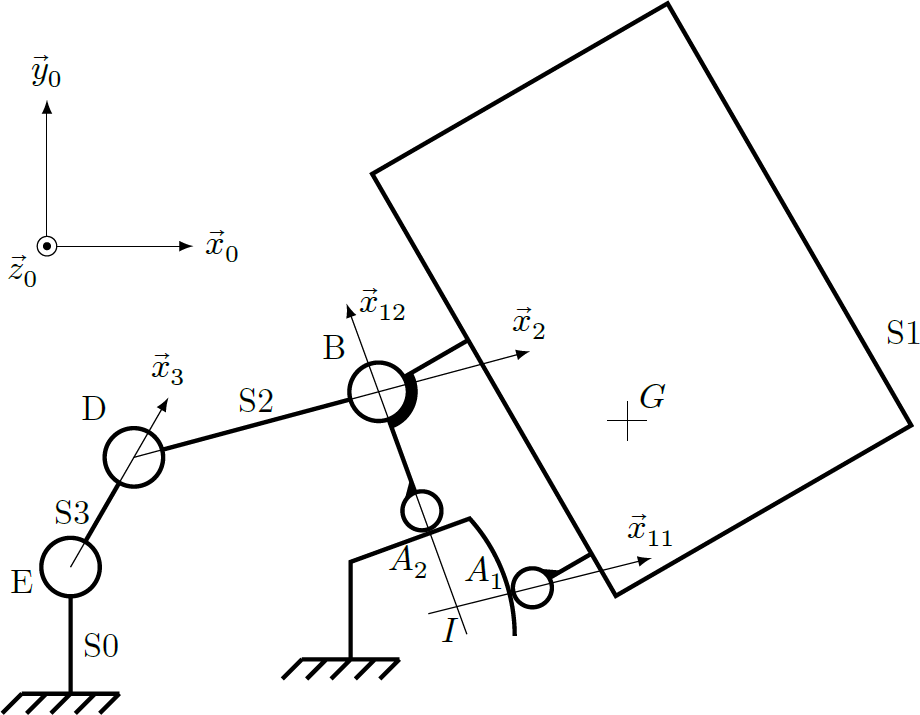
\includegraphics[width=.8\linewidth]{fig_04}
\caption{Aperçu du contrôle de $b_{\%}$. \label{Cy_11_Ch_03_PFS_3D_TD_01_fig_04}}
\end{marginfigure}


\begin{marginfigure}
\centering
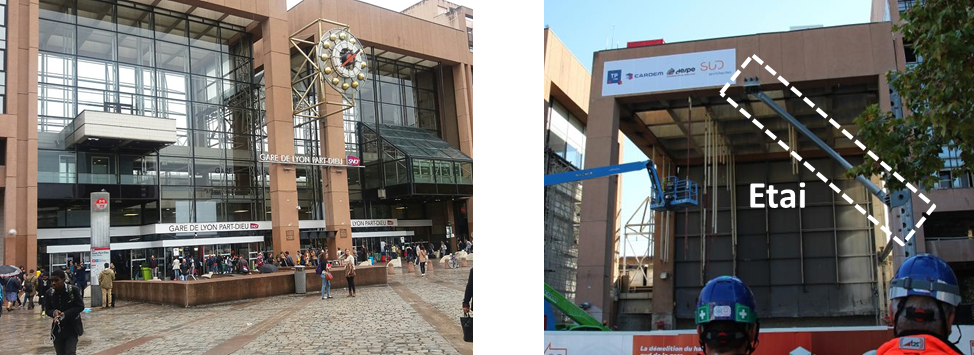
\includegraphics[width=\linewidth]{fig_03}
\caption{Exigence 1.2. \label{Cy_11_Ch_03_PFS_3D_TD_01_fig_03}}
\end{marginfigure}

Pour prévenir le basculement de la foreuse, l'opérateur peut observer dans un coin de son écran : le pourcentage $b_{\%}$ d’atteinte de la posture critique de basculement pour 
une orientation de tourelle donnée (figure \ref{Cy_11_Ch_03_PFS_3D_TD_01_fig_04}). 

 Afin d'assurer la stabilité de l'engin, on cherche à satisfaire l'exigence 1.2 (figure \ref{Cy_11_Ch_03_PFS_3D_TD_01_fig_03}).
 
\begin{figure}
\centering
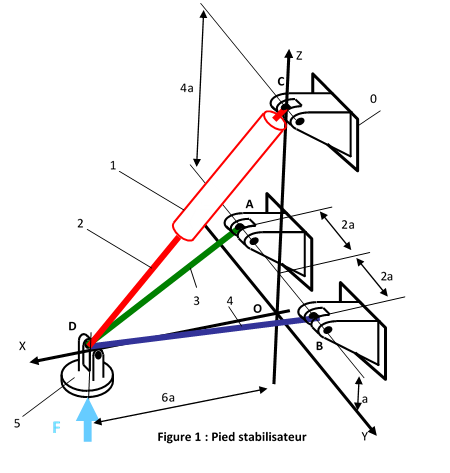
\includegraphics[width=.8\linewidth]{fig_02}
\caption{Paramétrage mécanique \label{Cy_11_Ch_03_PFS_3D_TD_01_fig_02}}
\end{figure}

Le paramétrage mécanique est donné sur la figure \ref{Cy_11_Ch_03_PFS_3D_TD_01_fig_02} : 
\begin{itemize}
\item \textbf{0} le sol, \textbf{S1} le châssis de la foreuse, \textbf{S2} sa tourelle et son mât et \textbf{S3} l’ensemble \{table de forage + outil\} ; 
\item $\rep{0} = \repere{O}{x}{y}{z}$ le repère attaché aux solides \textbf{S0} et \textbf{S1}; 
\item $\mathcal{B}_2=\base{x_2}{y_2}{z_2}$ la base attachée aux solides \textbf{Sé} et \textbf{S3} telle que $\angl{x}{x_2}=\theta$ où $\theta$ est connu ;
\item $\Sigma = $ \textbf{\{S1, S2, S3\}} l’ensemble de la foreuse, de centre de gravité $G$ tel que $\vect{OG} = r \vx{2} +  z_G \vect{z}$;
\item $M = \SI{186,5}{tonnes}$ la masse de l’ensemble $\Sigma$ et $m =\SI{18}{tonnes}$ la masse de \textbf{S3} seul ; 
\item $2F_w \vect{z}$ connu, l’effort du câble d’avance sur \textbf{S3}. La masse du câble est négligée dans la suite ; 
\item $\indice{F}{sol}\vect{z}$, inconnu, l’effort de forage du sol \textbf{0} sur l’outil de forage \textbf{S3} au point $F$, connu, défini par $\vect{OF}=R\vx{2}$;
\item $-g\vect{z}$  où $g = \SI{9,8}{m.s^{-2}}$, l’accélération de la pesanteur terrestre.
\end{itemize}

On modélise ici les contacts entre le sol et la foreuse\textbf{par des contacts ponctuels}  :
$F_g \vect{z}$, (respectivement  $F_d \vect{z}$) inconnu, l’effort du sol 0 sur S1, supposé ponctuel au centre $I$ (respectivement  $J$) de la surface de contact entre la chenille gauche $cg$ (respectivement  $c_d$) et le sol tel que $||\vect{OI}|| = a=\SI{2,1}{m}$ (respectivement  $||\vect{OJ}|| = a=\SI{2,1}{m}$).


\question{En appliquant le principe fondamental de la statique en $O$ à l’isolement de votre choix, donner l’expression de $\indice{F}{g}$ et de $\indice{F}{d}$ en fonction des données connues du système, de $\theta$ et de $\indice{F}{sol}$. }
\ifprof
\begin{corrige}
\paragraph*{On isole $\Sigma$.}

\paragraph*{BAME}
\begin{itemize}
\item action du sol en $I$;
\item action du sol en $J$;
\item pesanteur en $G$;
\item l'effort du sol sur l'outil. 
\end{itemize}

\end{corrige}
\else
\fi
Le problème étant symétrique pour $\theta \in \left[-\dfrac{\pi}{2};\dfrac{\pi}{2}\right]$(tourelle orientée à droite) et $\theta \in \left[\dfrac{\pi}{2};\dfrac{3\pi}{2}\right]$ (tourelle orientée à gauche), on n’étudie par la suite que le basculement statique à droite. 

\question{ Donner la condition en effort pour laquelle il y a basculement statique à droite. En absence d’effort de forage, en déduire la condition sur la position $\left(r,\theta\right)$ du centre de gravité $G$ pour laquelle le basculement à droite est alors évité.}
\ifprof
\begin{corrige}
\end{corrige}
\else
\fi

\question{Interpréter physiquement ce résultat et montrer que $b_{\%}$ peut être, dans ce cas, approximé par : $b_{\%} = 100\dfrac{\left| r\cos \theta \right|}{a}$.}
\ifprof
\begin{corrige}
\end{corrige}
\else
\fi

\begin{marginfigure}
\centering
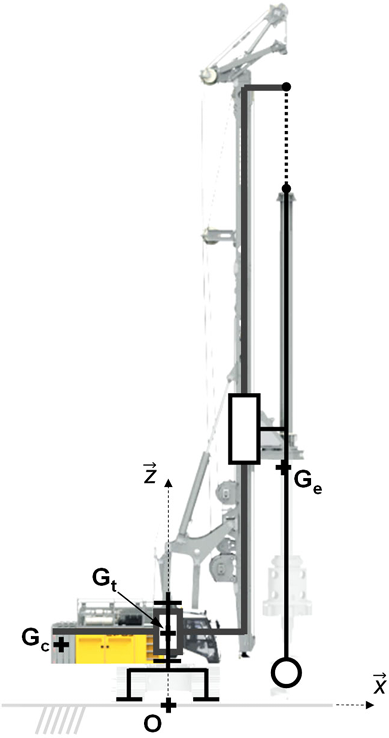
\includegraphics[width=\linewidth]{fig_05}
\caption{ Position des centres 
de gravité des différents solides. \label{Cy_11_Ch_03_PFS_3D_TD_01_fig_05}}
\end{marginfigure}

On désire dimensionner le nombre de contrepoids de 8 tonnes à 
placer à l’arrière de la tourelle pour que, en l’absence de forage 
et en extension maximale, l’exigence 1.2 d’équilibrage statique 
initial soit respectée même dans le pire des cas où la tourelle est 
pleinement orientée à droite ($\theta=0\degres$). Dans cette posture, le 
schéma de la figure \ref{Cy_11_Ch_03_PFS_3D_TD_01_fig_05} illustre où se situent, dans le même plan, 
les centres de gravité des différents éléments de la machine :  
\begin{itemize}
\item $G_t$ est le centre de gravité de la tourelle et du châssis. La 
masse de cet ensemble $S_t$ est notée $m_t = \SI{44,7}{tonnes}$ ; 
\item $G_e$ est le centre de gravité de tous les équipements mobiles 
(tige Kelly, potences, vérins, mât, table de forage, outillage, 
terre à évacuer), positionnés dans la configuration la plus 
défavorable. La masse de cet ensemble Se est notée 
$m_e = \SI{48,8}{tonnes}$; 
\item $G_c$ est le centre de gravité des contrepoids. Il y a $n_{cp}$ 
contrepoids de masse totale $m_c = n_{cp}\cdot m_1$, où $m_1 = \SI{8}{tonnes}$
est la masse d’un seul contrepoids; 
\item l’accélération de la pesanteur est notée : $\vect{g}=-g\vect{z}=-9,8\vect{z}$
(en \si{m/s^2}).
\end{itemize} 
On note (en mètres) : $\vect{OG_t}=2,2\vect{z}$, $\vect{OG_e}=4,4\vect{x}+13\vect{z}$; $\vect{OG_c}=-4,3\vect{x}+2,3\vect{z}$. On fait l'hypothèse que $\vect{OG_c}$ reste identique, indépendamment du nombre de contrepoids. 

\question{Exprimer la coordonnée sur $\vect{x}$, notée $r$, du centre de gravité $G$ total de la machine en fonction des paramètres connus et de $n_{cp}$. En déduire le nombre $n_{cp}$ minimum de contrepoids pour respecter l’exigence 1.2. }
\ifprof
\begin{corrige}
\end{corrige}
\else
\fi